\chapter{Flutter}

\section{Mobile Developement Tiers} \label{section::other_architectures}
\subsection{Web Apps and Progressive Web Apps}
Web apps are applications run and rendered in the browser. The underlying technologis are HTML, CSS and JavaScript with popular frameworks 
used for the development process such as Angualar (ref), React.js (ref) and Vue.js (ref). Web apps rely on the Browser and an internet connection.
They do not have direct access to hardware capabilites such as the camera or the file system.\\
Progressive Web Apps (PWAs) function similarly to web apps but provide additional capabilities such as offline use, locally cached data, 
push notifications, and the ability to add them to the home screen.

\subsection{Hybrid Apps}
Hybrid Apps utilize the same technologies as web apps, but they are rendered in a platform web view. Additionally they provide the ability to 
interact with native APIs through a platform bridge (see \ref{fig:hybrid_architecture}). 
Popular framework choices for building Hybrid Apps include Ionic and Cordova 
Hybrid apps unlike web apps are shippable to official stores.


\begin{figure}
    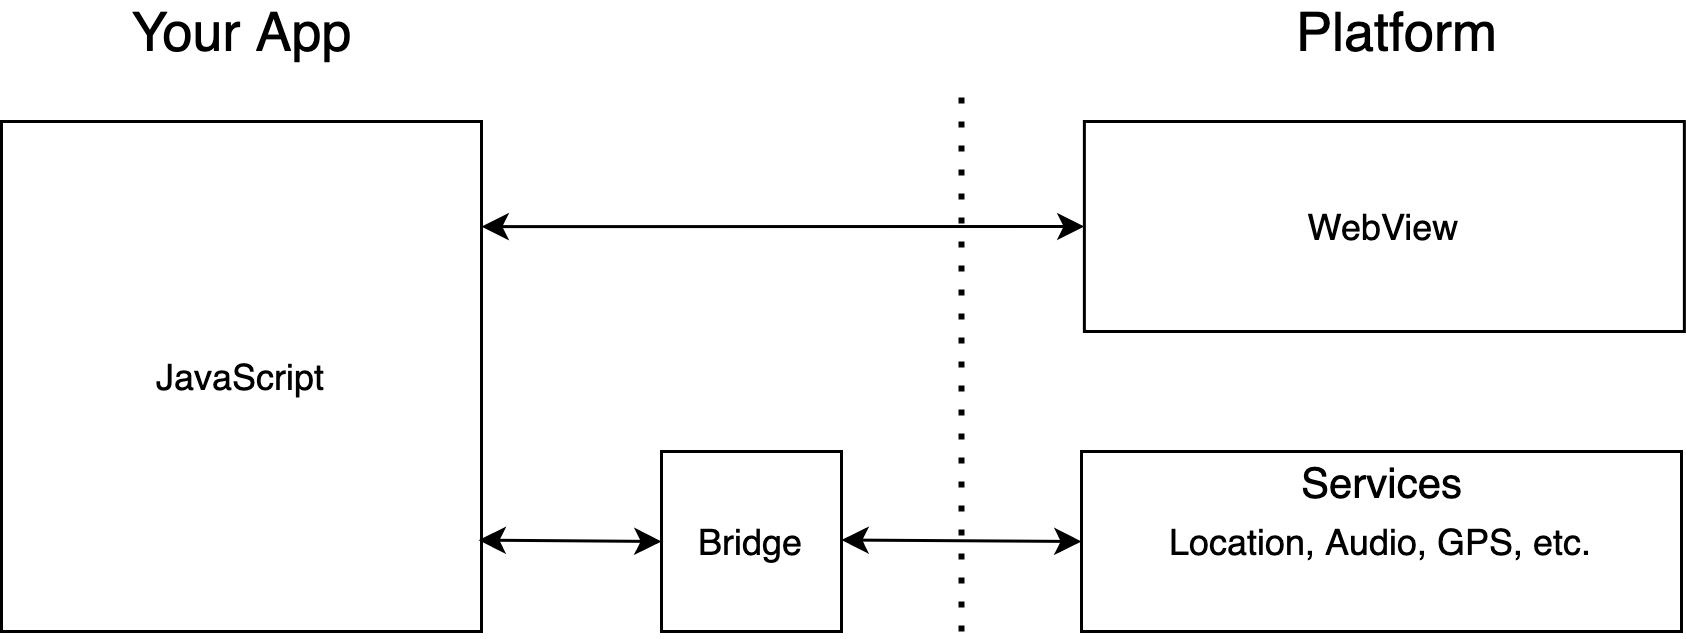
\includegraphics[width=\linewidth]{images/architectures/hybrid_architecture.png}
    \caption{Hybrid architecture (image to be replaced).}
    \label{fig:hybrid_architecture}  (ref: https://www.freecodecamp.org/news/a-deeply-detailed-but-never-definitive-guide-to-mobile-development-architecture-6b01ce3b1528/)
\end{figure}

\subsection{Web Native Apps}
Web Native Apps which are built with frameworks such as React Native (ref) or Native Script (ref) utilize the OEM components instead of web views.
This is achieved by using JavaScript calls to a platform bridge which transpiles the JavaScript code into native platform code (see \ref{fig:web_native_architecture}). 
The views are thus in Web Native Apps rendered with native technologies.

\begin{figure}
    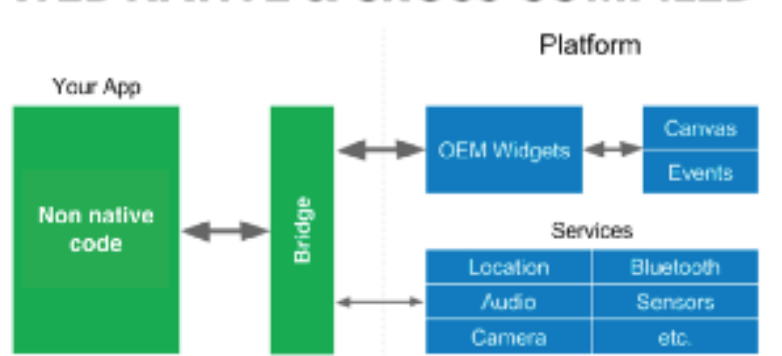
\includegraphics[width=\linewidth]{images/architectures/native_web_app_architecture.png}
    \caption{Web Native and Cross Compiled Architecture (image to be replaced).}
    \label{fig:web_native_architecture}
\end{figure}

\subsection{Cross Compiled Apps}
Cross Compiled Apps utilize a compiled programming language such as C\# (used for Xamarin) to generate byte or machine code which is then executed 
on the host platform. This machine code performs similar actions as web native apps in that platform APIs and OEM widgets are called (see \ref{fig:web_native_architecture}).
Flutter can also be classified as a cross compiled architecture. However, Flutter ships its own widgets and rendering engine instead of relying on
the host platform (see \ref{fig:flutter_architecture}). These technicalities will be explained in Section \ref{section::flutter_architecture}.

\begin{figure}
    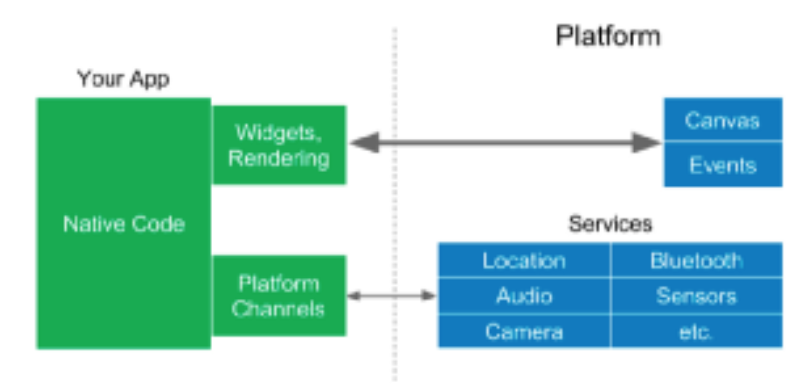
\includegraphics[width=\linewidth]{images/architectures/flutter_architecture.png}
    \caption{Flutter Architecture (image to be replaced).}
    \label{fig:flutter_architecture}
\end{figure}

\subsection{Native Mobile Applications}
Native applications directly communicate with the OEM components and APIs which are part of the operating system and thus tightly integrated into the platform.
Making full use of hardware and software integration, native apps yield the highest performance and user experience.

\begin{figure}
    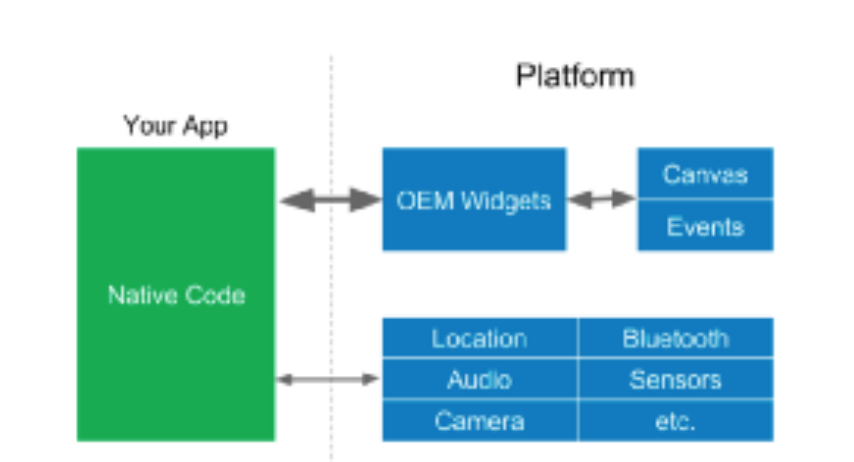
\includegraphics[width=\linewidth]{images/architectures/native_architecture.png}
    \caption{Native Mobile Architecture (image to be replaced).}
    \label{fig:native_architecture}
\end{figure}

\section{Flutter Framework Architecture} \label{section::flutter_architecture}
Flutter's framework architecture is composed of three distinct layers: framework, engine and embedder. The framework acts as the top most layer which 
app developers interact with. It features the widgets, animation and gestures API as well as platform specific UI components delivered through
the Material (Android) and Cupertino (iOS) package.
\\
Below the framework layer lies the engine which unlike the framework isn't written in Dart, but in C and C++. Presumably, this design choice has been 
made to easily allow the production of native binaries. This act of cross-compilation is Flutter's technical value proposition to increase execution performance as stated in 
Section \ref{section:introduction}. The engine layer includes Skia - a 2D graphics rendering engine which is also used in the Chrome web browser.
\\
At the bottom lies the embedder layer. Its sole purpose is to integrate the Flutter application into the platform-specific environment
by providing native plugins and event loop interoperation. 
Additionally, app package formatting is provided in the same way as for native apps. 
The host operating is thus not able to differentiate between a Flutter and a natively written app.\\ 
Flutter aims to minimize application size as it's already shipping the entire framework including the rendering engine with each app which amounts
to approximately 4.5 mb (https://flutter.dev/docs/resources/faq). Common app platform plugin functionality like camera access or webview 
interaction are extracted in separate packages. Networking, animations or other platform agnostic functionality is also bundled in packages. 

\begin{figure}
    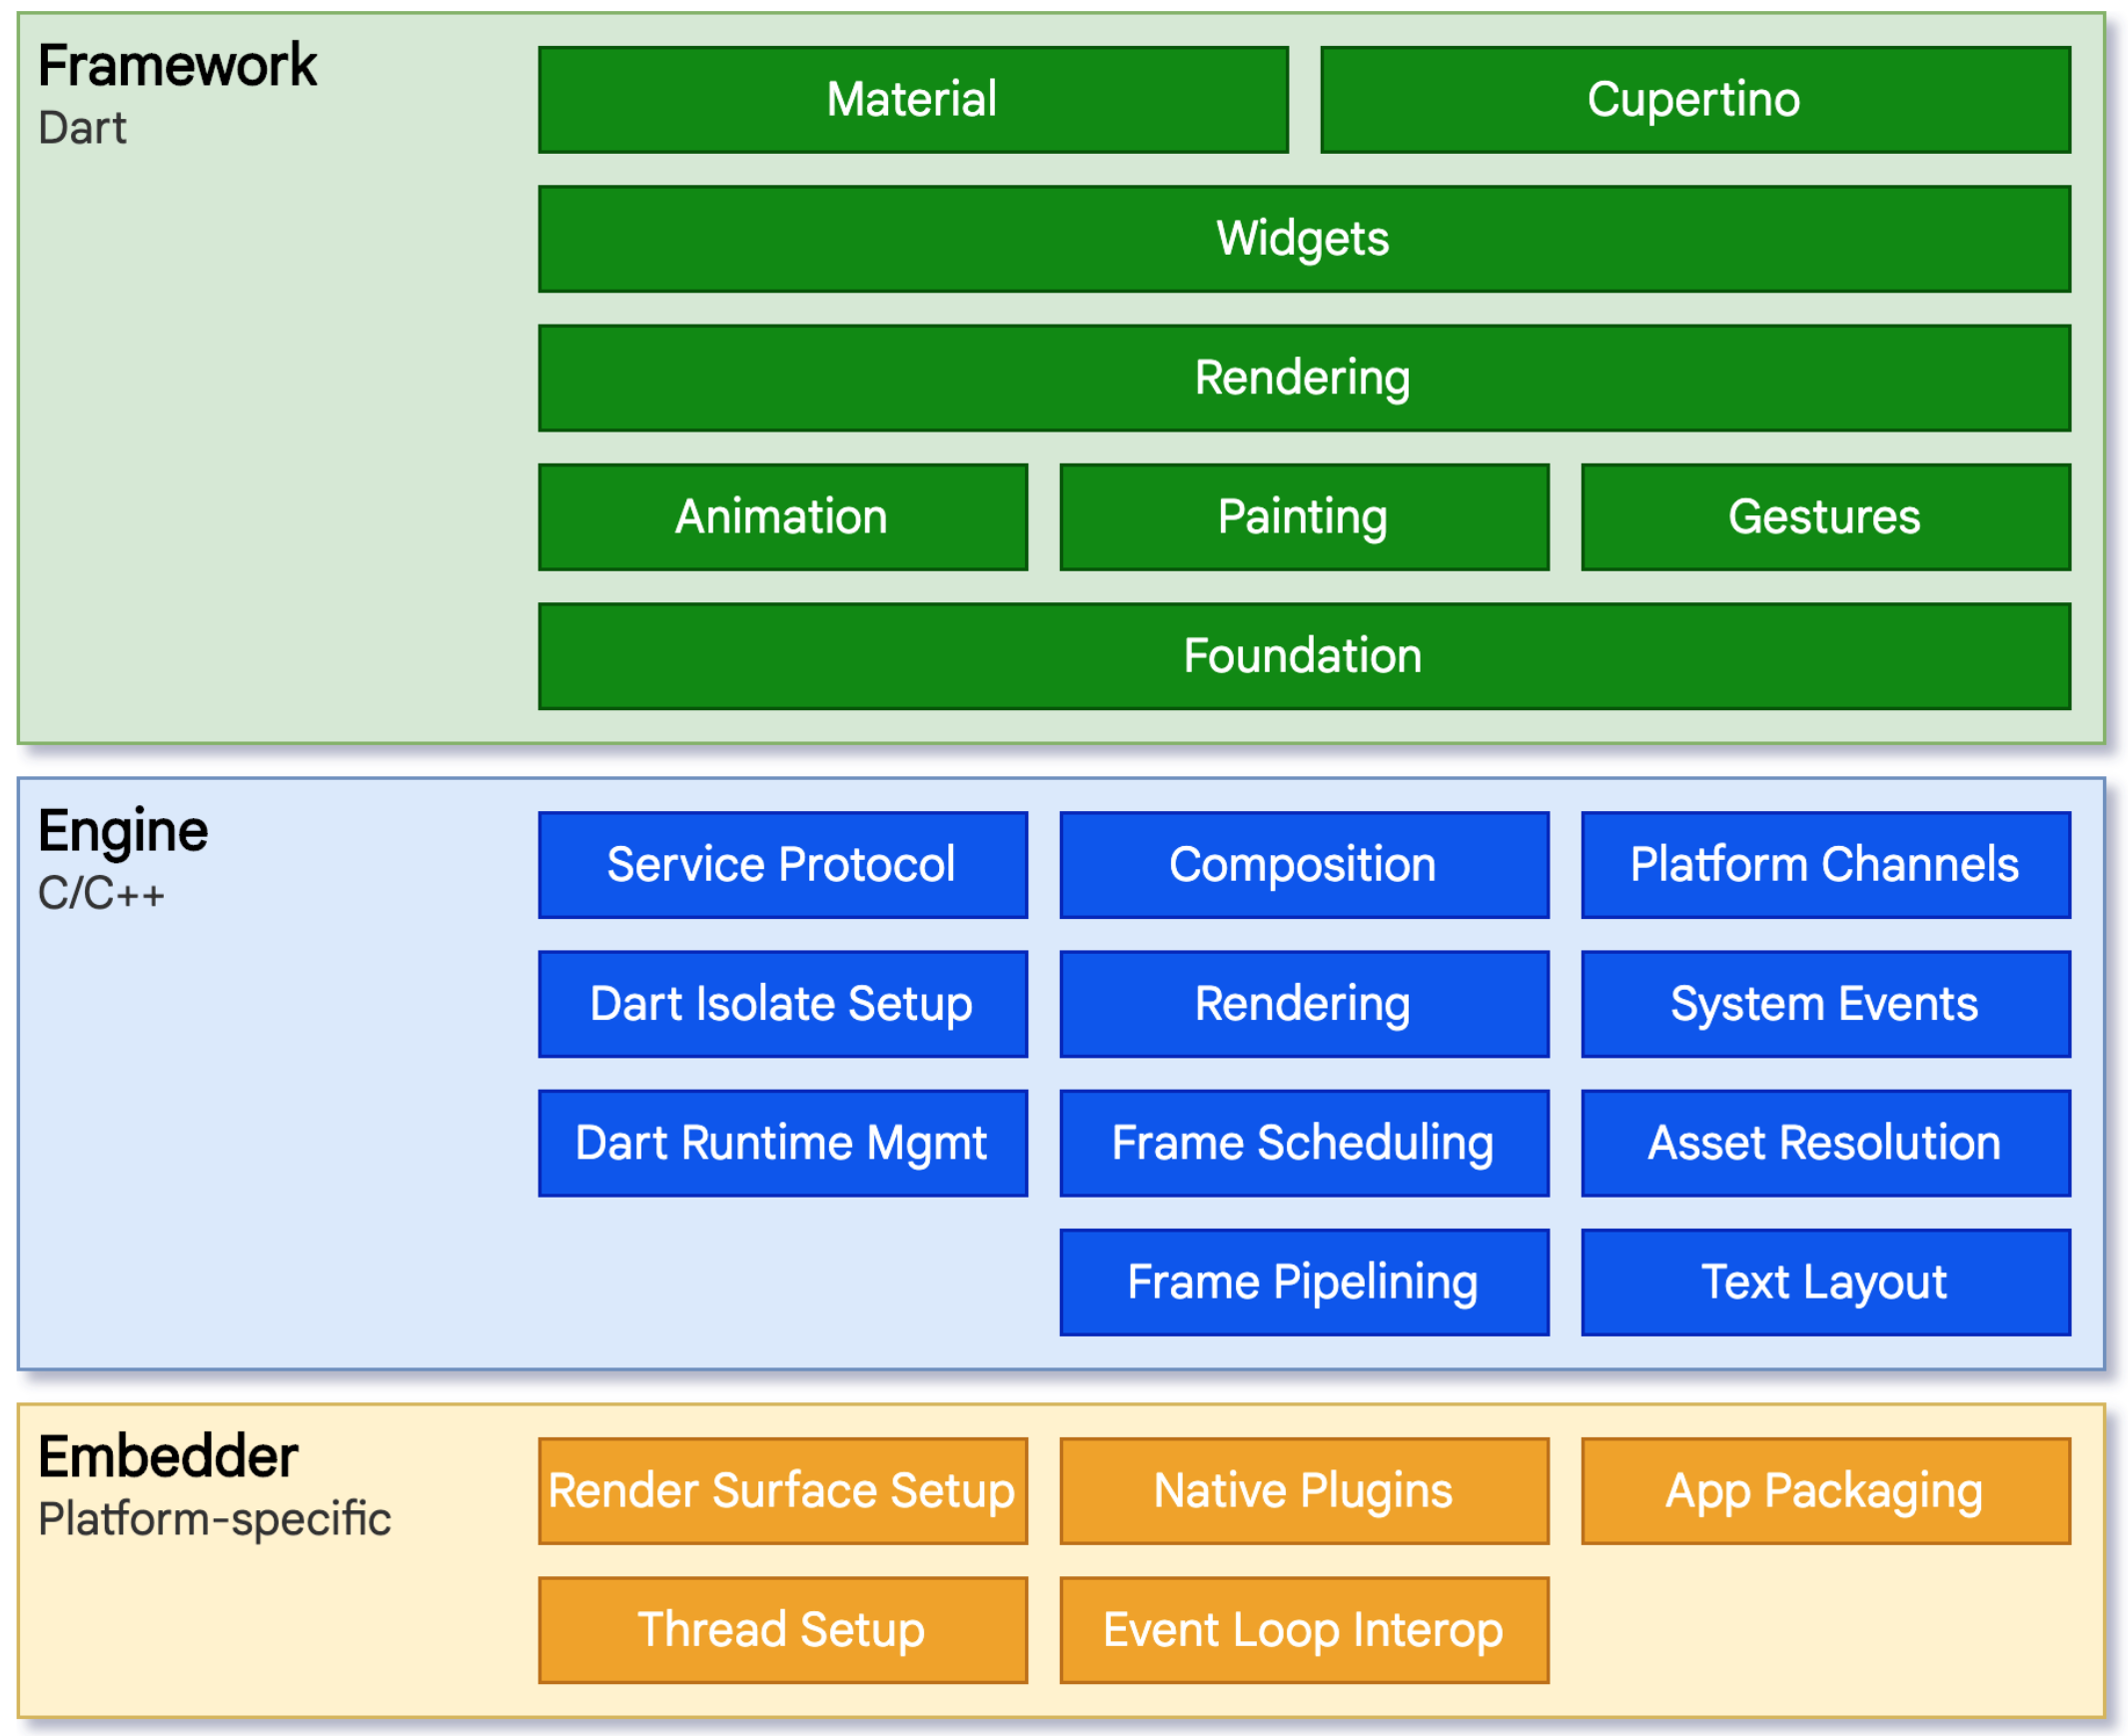
\includegraphics[width=\linewidth]{images/flutter_layered_architecture.png}
    \caption{Flutter's Layered Architecture (ref to include https://flutter.dev/docs/resources/architectural-overview).}
    \label{fig:native_architecture}
\end{figure}


\subsection{Programming Language and Compilation}
Flutter apps are written in Dart an multiparadigm programming language syntactically similar to Java. (https://dart.dev/overview\#language)

During Flutter development, apps run in the Dart Virtual Machine with JIT compilation. This offers stateful hot reload which allows reload changes without needing 
to fully recompile the app leading faster development iteration.
For release purposes, Flutter applications are Ahead-of-Time compiled into native machine code including the Intel x86 and ARM instruction sets.
(https://flutter.dev/docs/resources/architectural-overview).


\subsection{Rendering and UI State}
Flutter apps are fundamentally composed of widgets which declare structural, stylistic and layout elements for building the user interface. 
Each widget may have 0, 1 or multiple children which in turn create a tree structure of parent-child relationships. 
For example, a Column which has the purpose of laying out its children vertically has both a Text and an Image as its children. Both the Text,
and Image widgets have no children and represent the leaf nodes in the tree. The Column is an invisible structural layout element while Text and 
Image are stylistic.
\footnote{Technically both Text and Image do have an implicit single child widget which is created by the framework.}
The entry point of every Flutter app is either a 'MaterialApp' or 'CupertinoApp' widget which also marks the root of the tree.
Based on this tree structure Flutter can determine where and how elements should be drawn on screen, and instruct its graphics engine accordingly.\\
This concept alone is not yet sufficient to enable modern mobile applications with complex UI changes or animations 
based on asynchronous events like user interaction. 
Widgets are mappings from state to a UI representation. When the state changes during runtime Flutter creates a new widget tree, 
diffs it against the old one and then redraws only its changes to the screen.
This declarative approach simplifies UI development in the sense that the developer does not need to keep track of UI state which can grow exponentially
with the increase of UI components on screen. 

\subsection{Method Channels}
To utilize platform functionality like camera access, geolocation or other sensor data, Flutter communicates with the platform's native APIs via 
method channels (see architecture diagram). Common functionality is already provided by Flutter and third party packages, but custom platform channel
functionality may be implemented as required. (reference Flutter doucmentation...)

\section{Flutter's Limitations}
Unlike other cross-platform frameworks, Flutter doesn't use OEM components, but its own components instead (widgets).\\
When the underlying OEM component of the host platform changes with an OS update, Flutters' framework needs to updated to resemble this new 
functionality. Flutter always has to continuously replicate these changes in their framework layer. As Google is using Flutter itself in multiple 
production apps (cite something), the company has an incentive to swiftly replicate OS features. Additionally, since Google also owns Android, 
coordination may be easier and not as surprising.
The benefit though is that once the new widget is rebuilt in Flutter it can even be shipped to older operating systems.